\documentclass[12pt]{article}

% --- Packages ---
\usepackage{amsmath, amssymb}
\usepackage{graphicx}
\usepackage{geometry}
\usepackage{hyperref}
\usepackage{ifthen} % for safe graphics include
\pdfstringdefDisableCommands{%
  \def\theta{theta}%
  \def\Theta{Theta}%
  \def\mathbb#1{#1}%
  \def\mathbf#1{#1}%
  \def\mathrm#1{#1}%
}
% after \usepackage{graphicx,hyperref,ifthen}
\graphicspath{{figs/}{../figs/}} % search both source and build-relative figs
\newcommand{\maybeincludegraphics}[2][]{%
  \IfFileExists{#2}{\includegraphics[#1]{#2}}{%
    \fbox{\parbox{0.85\linewidth}{\centering \textbf{Missing figure:} \texttt{\detokenize{#2}}}}%
  }%
}


% --- Page setup ---
\geometry{margin=1in}

% --- Graphics paths ---
% Look both in ./figs (when running from paper/) and ../figs (when output-directory=build/)
\graphicspath{{figs/}{../figs/}}


% --- Title ---
\title{Foundations of the X--$\theta$ Framework: $Q=\mathbb{R}^3 \times S^1$ and Testable Predictions}
\author{Divyang Panchasara}
\date{September 2025}

\begin{document}

\maketitle

% --- Sections ---
\begin{abstract}
I introduce the X--$\theta$ framework, extending particle configuration space to
$Q=\mathbb{R}^3\times S^1$ via an internal vibration angle $\theta$.
I motivate the structure, develop a minimal formalism, and derive testable predictions:
a $\theta$-phase contribution in interferometry, photoelectric thresholds modified by internal energy exchange,
possible softening of geodesic pathologies near compact objects, and gravitational-wave birefringence.
I propose tabletop experiments and provide open simulations for reproducibility.
\end{abstract}

\section{Motivation and Origin}

This framework grew out of my own journey in learning. While self-studying AI/ML, I
wanted to refresh my knowledge of statistics and searched for good video lectures online.
By chance, I encountered a statistics lecture by Dr.~Ashwin Joy (IIT Madras)
\cite{ashwinjoy_youtube} (who also happens to be my college best friend!), whose clarity rekindled my interest in mathematical thinking.
From there I explored \textbf{NPTEL} and \textbf{IITM online courses}, eventually reaching
Prof.~V.~Balakrishnan’s celebrated lectures on quantum mechanics
\cite{balakrishnan_qm_series}. 

One particularly striking talk, \emph{``Electron, a wave or a particle?''}
\cite{balakrishnan_wave_particle}, revived the century-old puzzle:

\begin{quote}
\emph{Is an electron or photon a particle, or a wave?}
\end{quote}

Quantum mechanics teaches that it is neither purely particle nor purely wave, but a
hybrid object. To me, this duality felt like saying: ``it is neither man nor woman, but
something in between''---a metaphor for quantum indeterminacy.

\subsection{Classic Puzzles}

This puzzle echoes two landmark experiments:

\begin{itemize}
  \item \textbf{Double slit experiment.} Electrons and photons produce interference fringes,
        acting like waves \cite{feynman_double_slit}.
  \item \textbf{Photoelectric effect.} The same photons eject electrons in discrete packets,
        acting like particles \cite{einstein_nobel}.
\end{itemize}

Quantum mechanics accounts for both, but its \emph{probabilistic interpretation} left
Einstein uneasy. General relativity, by contrast, is deterministic and geometric. Their
clash is not superficial---it runs deep.

\section{Our Motivation}

We propose that every particle carries not only a spatial coordinate
$X \in \mathbb{R}^3$ but also an internal cyclic coordinate $\theta \in S^1$---a vibration
angle. The configuration space is thus extended to

\[
Q = \mathbb{R}^3 \times S^1.
\]

\textbf{Analogy:} Imagine a bike on a mountain road. The road represents spacetime $X$,
the handlebar angle represents $\theta$. You may return to the same location on the road,
but the handlebars can end up rotated. This leftover orientation is a \emph{holonomy}.
Likewise, a particle can return to the same point in spacetime but with a shifted internal
phase. That phase shift can leave observable traces, even in field-free conditions.

This framework---the \textbf{X--$\theta$ theory}---aims to provide a common language for
phase phenomena, from Aharonov--Bohm effects to dark photon searches, while remaining
simple enough to teach at an undergraduate level.

\section{Where QM and GR Disagree}

Modern physics rests on two great pillars:

\begin{itemize}
  \item \textbf{Quantum Mechanics (QM)}: The probabilistic theory that governs atoms,
        molecules, and semiconductors \cite{wiki_qm}.
  \item \textbf{General Relativity (GR)}: The geometric theory of curved spacetime that
        governs black holes and the expanding universe \cite{wiki_gr}.
\end{itemize}

Each works spectacularly in its own domain, yet when pushed together, they crack. Key
tensions include:

\begin{enumerate}
  \item \textbf{Singularities.} GR predicts infinite curvature (black holes, Big Bang),
        while QM forbids infinities \cite{padmanabhan_cc}.
  \item \textbf{Wave--particle duality.} QM formally explains interference and particle
        detection, but gives little intuition about what oscillates.
  \item \textbf{Gravitational phase ambiguity.} Should a quantum wavepacket’s phase in
        curved spacetime follow geodesic length (GR) or Schrödinger evolution (QM)?
  \item \textbf{Measurement vs determinism.} QM invokes probabilities and collapse, GR
        assumes definite trajectories.
  \item \textbf{Vacuum energy crisis.} QFT predicts a vacuum energy $10^{120}$ times
        larger than what GR infers from the cosmological constant.
\end{enumerate}

These contradictions suggest that our notion of a ``particle'' is incomplete and that a
richer framework is needed to bridge QM and GR.
 % Classic Puzzles & Open Problems
\input{sections/09_related_work} % Related Work & Originality
\section{The X--$\theta$ Framework}

Each particle carries two degrees of freedom:
\begin{itemize}
  \item A center coordinate $X \in \mathbb{R}^3$ (its spatial position in ordinary space).
  \item An internal vibration $\theta \in S^1$ (a cyclic, angle-like variable).
\end{itemize}

Thus the configuration space is extended to
\begin{equation}
Q = \mathbb{R}^3 \times S^1 .
\end{equation}

This means that in addition to position, every particle carries an internal ``handlebar angle'' 
that can accumulate holonomy. The resulting framework---the \textbf{X--$\theta$ theory}---is minimal, geometric, 
and falsifiable.

\subsection{Analogy: Bike in the Nilgiris}
Imagine a bike moving along a winding mountain road:
\begin{itemize}
  \item The road corresponds to spacetime ($X$).
  \item The handlebar orientation corresponds to $\theta$.
\end{itemize}
A rider may return to the same location on the road, yet the handlebar can be rotated.
This mismatch is a \emph{holonomy}, and it illustrates how $\theta$ can produce observable
effects even when the center coordinate $X$ returns to its original position.  

\subsection{Conceptual Foundations}

\subsubsection*{Center $X$ (the base)}
The center $X$ denotes the usual position of a particle in space. In experiments, this is what
I measure directly: trajectories, scattering angles, interference patterns.  
I treat $X \in \mathbb{R}^3$ for nonrelativistic models, or as a curved 3-manifold in relativistic extensions.

\subsubsection*{Vibration $\theta$ (the fiber)}
The vibration $\theta$ is an internal, periodic coordinate:
\[
\theta \in S^1 .
\]
It is not an extra spatial dimension, but a compact ``clock'' variable attached to each point in space.
Its conjugate momentum $p_\theta = -i\hbar \partial_\theta$ is quantized in integer multiples of $\hbar$, 
reflecting the periodicity. This means that particles can exchange discrete quanta of internal energy 
through the $\theta$ channel.

\subsubsection*{One connection, many forces}
On the full space $Q = \mathbb{R}^3 \times S^1$, I introduce a single gauge connection:
\begin{equation}
A = A_i(x,\theta)\, dx^i + A_\theta(x,\theta)\, d\theta, \quad i=1,2,3,
\end{equation}
with curvature
\begin{align}
F = dA 
&= (\partial_i A_j - \partial_j A_i)\, dx^i \wedge dx^j \quad \text{(center--center sector)} \\
&\quad + (\partial_i A_\theta - \partial_\theta A_i)\, dx^i \wedge d\theta 
\quad \text{(center--vibration sector)} .
\end{align}

\begin{itemize}
  \item The $dx \wedge dx$ terms reproduce familiar spatial-field forces.
  \item The mixed $dx \wedge d\theta$ terms couple center motion to the internal phase $\theta$.
\end{itemize}

In this way, apparently distinct physical effects---Lorentz forces, holonomies, and 
fiber-driven drifts---arise as different projections of the same underlying curvature $F$.

\subsection{Connections to Prior Work}

While exploring these ideas, I also read research papers and reviews on several related directions:
\begin{itemize}
  \item \textbf{Extra U(1) sectors and kinetic mixing} (Holdom, Okun, Essig).
  \item \textbf{Aharonov--Bohm and geometric phases}.
  \item \textbf{Synthetic gauge fields in cold atoms}.
  \item \textbf{Interferometry with atoms and neutrons}.
  \item \textbf{Mass generation mechanisms and dark photon searches}.
\end{itemize}

Each of these threads provides valuable insight: hidden $U(1)$ fields suggest new interactions;
the Aharonov--Bohm effect shows that potentials are physical; cold-atom experiments engineer 
synthetic vector potentials; interferometry probes delicate phases; and dark photon searches 
bound new sectors.

My contribution is to \emph{visualize these disparate ideas through a single, unified lens}: 
the fiber holonomy of $\theta$. The $U(1)_\theta$ connection makes the analogy concrete and 
gives a natural way to design tabletop tests that isolate the new effects.
 % The X-theta Framework
\section{Analogies for Understanding}

\subsection{Gyroscope}
A gyroscope has both a spatial location and an internal spin orientation. The
latter is invisible in ordinary coordinates but crucial for dynamics.

\subsection{Fiber Bundle}
The mathematical structure resembles a fiber bundle with base space
$\mathbb{R}^3$ and fiber $S^1$. The $\theta$ coordinate behaves like an
internal gauge degree of freedom, similar to a $U(1)$ connection.

\subsection{Music Analogy}
A note has both pitch (analogous to $X$) and phase (analogous to $\theta$).
Two instruments playing the same note can interfere differently depending on
their phase.
 % Analogies
\section{Mathematical Formalism}
\label{sec:math_formalism}

Having defined the configuration space $Q=\mathbb{R}^3\times S^1$, I now construct the
dynamics for the center $X$ and the internal angle $\theta$. The core point is simple:
on the compact fiber $S^1$ there is a unique quadratic kinetic term, which introduces an
\emph{effective} moment of inertia $I$ in the internal space. This yields the
Hamiltonian contribution $p_\theta^2/(2I)$ and remains valid for both massive and
massless probes.

\subsection{Classical worldline formulations}

\subsubsection{Massive probes (proper-time gauge)}
For a particle of rest mass $m$ moving in a (possibly curved) background with metric $g_{\mu\nu}$,
an economical reparameterization-invariant action is
\begin{equation}
S_\text{massive}=\int d\tau\left[
 -m\sqrt{-g_{\mu\nu}(x)\,\dot x^\mu \dot x^\nu}
 + q A_\mu(x,\theta)\,\dot x^\mu
 + q A_\theta(x,\theta)\,\dot\theta
 + \frac{I}{2}\,\dot\theta^2
\right],
\label{eq:Smassive}
\end{equation}
where $I>0$ is the internal (fiber) moment of inertia, $q$ is a universal coupling to the
single connection on $Q$, and dots denote $d/d\tau$.

Varying $x^\mu$ and $\theta$ gives
\begin{align}
m\,\frac{D u^\mu}{D\tau} &= q\,F^{(\theta)\,\mu}{}_{\nu}(x,\theta)\,u^\nu,
\qquad u^\mu\equiv \dot x^\mu,
\label{eq:centerEOM}
\\
\frac{d}{d\tau}(I\dot\theta) &= q\left(\partial_\theta A_\mu\,u^\mu+\partial_\theta A_\theta\,\dot\theta\right),
\label{eq:fiberEOM}
\end{align}
so the mixed curvature $F_{i\theta}=\partial_i A_\theta-\partial_\theta A_i$ sources angular momentum flow in the
$\theta$ channel. Stationary/axisymmetric backgrounds then imply drifts in energy and
angular momentum through the usual Killing charges.

\subsubsection{Massless probes (affine-parameter gauge)}
For photons (or other ultra-relativistic quanta), proper time is not available. I use a
first-order (phase-space) worldline with an affine parameter $\lambda$ and a Lagrange
multiplier $\lambda_x$ enforcing the null constraint:
\begin{equation}
S_\text{massless}=\int d\lambda\left[
 p_\mu \dot x^\mu - \frac{\lambda_x}{2}\,p^2
 + \frac{I}{2}\left(\frac{D\theta}{D\lambda}\right)^2
 + q A_\mu(x,\theta)\,\dot x^\mu
 + q A_\theta(x,\theta)\,\frac{D\theta}{D\lambda}
\right].
\label{eq:Smassless}
\end{equation}
The $p^2=0$ constraint decouples the center kinematics from the \emph{internal} rotor term,
which still contributes via $I$. Choosing laboratory time $t$ as a parameter and eliminating
constraints reproduces the same $\theta$-sector dynamics used below. Thus $I$ is an \emph{internal}
inertia, not a rest mass, and it consistently applies to both electrons and photons.

\subsection{\texorpdfstring{Canonical structure on $S^1$: why the Hamiltonian has $I$}{Canonical structure on S\^1: why the Hamiltonian has I}}
On a compact angle $\theta\sim\theta+2\pi$, rotational invariance fixes the kinetic term to
\begin{equation}
L_\theta=\frac{I}{2}\,\dot\theta^2 \quad\Longrightarrow\quad p_\theta=\frac{\partial L_\theta}{\partial \dot\theta}=I\dot\theta.
\end{equation}
The fiber Hamiltonian is therefore
\begin{equation}
H_\theta=\frac{p_\theta^2}{2I}.
\end{equation}
Minimal coupling to the $U(1)_\theta$ connection shifts $p_\theta\mapsto p_\theta-qA_\theta$, giving
\begin{equation}
H_\theta=\frac{1}{2I}\,\big(p_\theta-qA_\theta\big)^2.
\end{equation}
Quantizing $p_\theta\to -i\hbar\,\partial_\theta$ yields the operator form used in this paper:
\begin{equation}
\hat H_\theta=\frac{1}{2I}\,\big(-i\hbar\,\partial_\theta-qA_\theta\big)^2.
\label{eq:Htheta_op}
\end{equation}
Because $\theta$ is periodic, $\hat L_\theta=-i\hbar\partial_\theta$ has integer-spaced eigenvalues $\ell\hbar$,
so the internal spectrum forms discrete sidebands whose spacing scales like $\hbar^2/I$.

\paragraph{Field-theory (stiffness) origin of $I$.}
If a microscopic sector carries a compact phase $\phi$ with an effective time-kinetic stiffness $K$
(e.g.\ from a quadratic term $\tfrac{K}{2}\dot\phi^2$ in a collective coordinate truncation), then identifying
$\theta\equiv \phi$ immediately gives $I\equiv K$. This origin of $I$ is agnostic to whether the carrier
has rest mass; it is particularly natural for neutral atoms (Ramsey phase) and for photons
(polarization/global phase as a compact variable).

\subsection{\texorpdfstring{Quantum dynamics on $Q$}{Quantum dynamics on Q}}
Promoting the state to $\Psi(X,\theta,t)$, the Schrödinger equation is
\begin{equation}
i\hbar\,\partial_t \Psi=\hat H\,\Psi,
\end{equation}
with
\begin{equation}
\hat H=\frac{1}{2m}\,\big(-i\hbar\nabla_X-qA_X\big)^2
      +\frac{1}{2I}\,\big(-i\hbar\partial_\theta-qA_\theta\big)^2
      +V(X,\theta),
\label{eq:full_H}
\end{equation}
where the first term is omitted for strictly massless quanta in a center-of-energy frame, or treated in an
ultra-relativistic envelope approximation when convenient. The internal term
\eqref{eq:Htheta_op} remains the same, reflecting its purely \emph{fiber} origin.

\subsection{\texorpdfstring{Continuity equation on $Q$}{Continuity equation on Q}}
Probability conservation takes the form
\begin{equation}
\partial_t|\Psi|^2+\nabla_X\!\cdot J_X+\partial_\theta J_\theta=0,
\end{equation}
with gauge-covariant currents
\begin{align}
J_X&=\frac{\hbar}{m}\,\text{Im}(\Psi^\ast\nabla_X\Psi)-\frac{q}{m}\,A_X\,|\Psi|^2,\\
J_\theta&=\frac{\hbar}{I}\,\text{Im}(\Psi^\ast\partial_\theta\Psi)-\frac{q}{I}\,A_\theta\,|\Psi|^2.
\end{align}
A nonzero mixed curvature $F_{i\theta}=\partial_iA_\theta-\partial_\theta A_i$ transfers probability between the
center and the fiber channels (\emph{cross-Hall} pumping).

\subsection{How to measure I (massive or massless carriers)}
The internal level spacing is set by
\begin{equation}
\Delta E_\theta\sim \frac{\hbar^2}{I},
\end{equation}
so $I$ can be extracted by:
\begin{enumerate}
\item \textbf{Ramsey/Mach--Zehnder in the $\theta$-channel:} measure sideband spacing vs.\ drive frequency.
\item \textbf{Fringe offsets under null-EM:} fit the phase budget including $\tfrac{1}{2I}(-i\hbar\partial_\theta-qA_\theta)^2$.
\item \textbf{Cross-Hall drift:} calibrate transverse shifts $\Delta x\propto (\partial_xA_\theta)\,\Omega\,T_\text{int}$ while scanning $\Omega$.
\end{enumerate}
These methods are identical in form for electrons, neutrons, atoms, and photons; only the \emph{center}
kinematics differ.
 % Math Formalism
\section{Testable Predictions}\label{sec:predictions}

\subsection{Double Slit Residual Fringes}
The total phase includes:
\begin{equation}
\Delta\phi = \Delta\phi_{\text{path}} + \Delta\phi_\theta.
\end{equation}
Figure~\ref{fig:double-slit-sweep} shows simulated fringe shifts for a drive-locked $\theta$ modulation.

\begin{figure}[h]
  \centering
  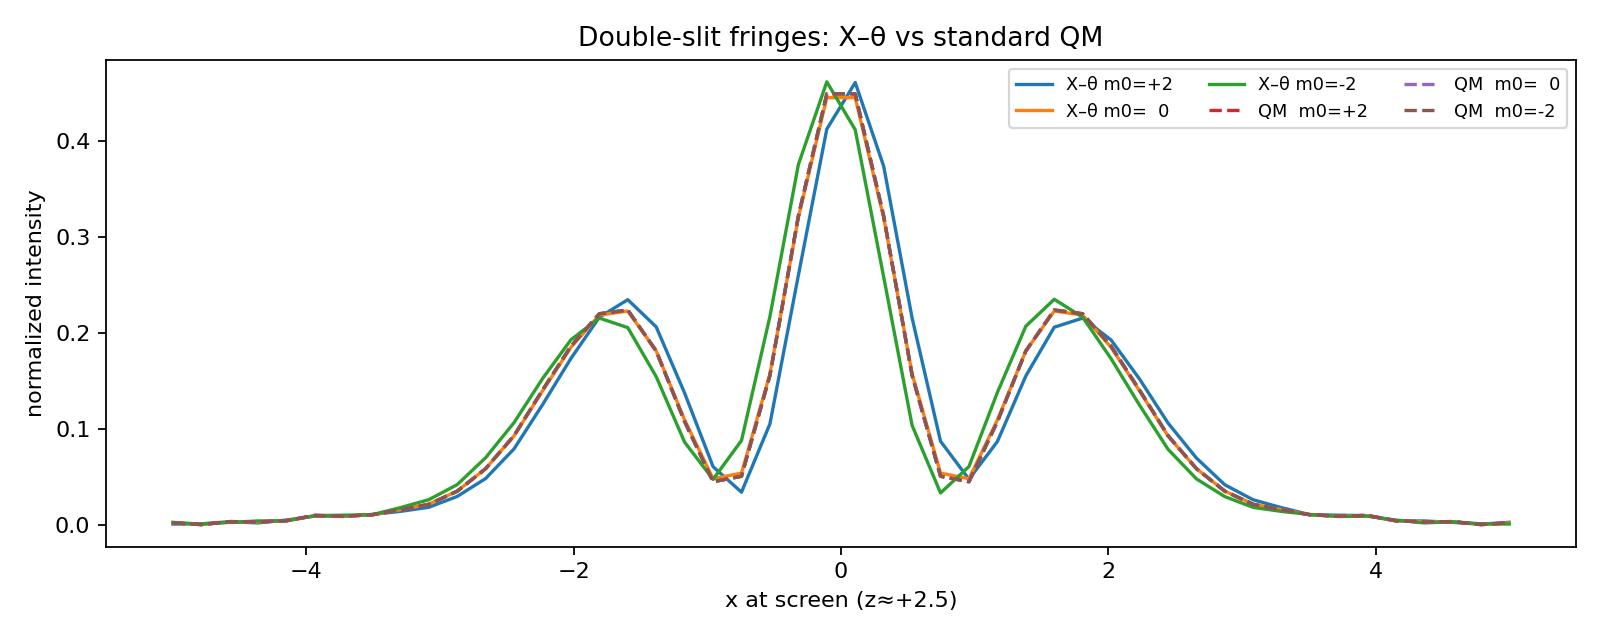
\includegraphics[width=0.85\linewidth]{double_slit_sweep.png}
  \caption{Predicted fringe shift vs $\theta$-drive amplitude and frequency (simulation).
  Null-EM conditions isolate $\Delta\phi_{\theta}$.}
  \label{fig:double-slit-sweep}
\end{figure}

\subsection{Photoelectric Effect Modifications}
Our framework predicts that $\theta$ introduces an internal quantized energy channel,
slightly shifting the classical cutoff frequency.

\begin{figure}[h]
  \centering
  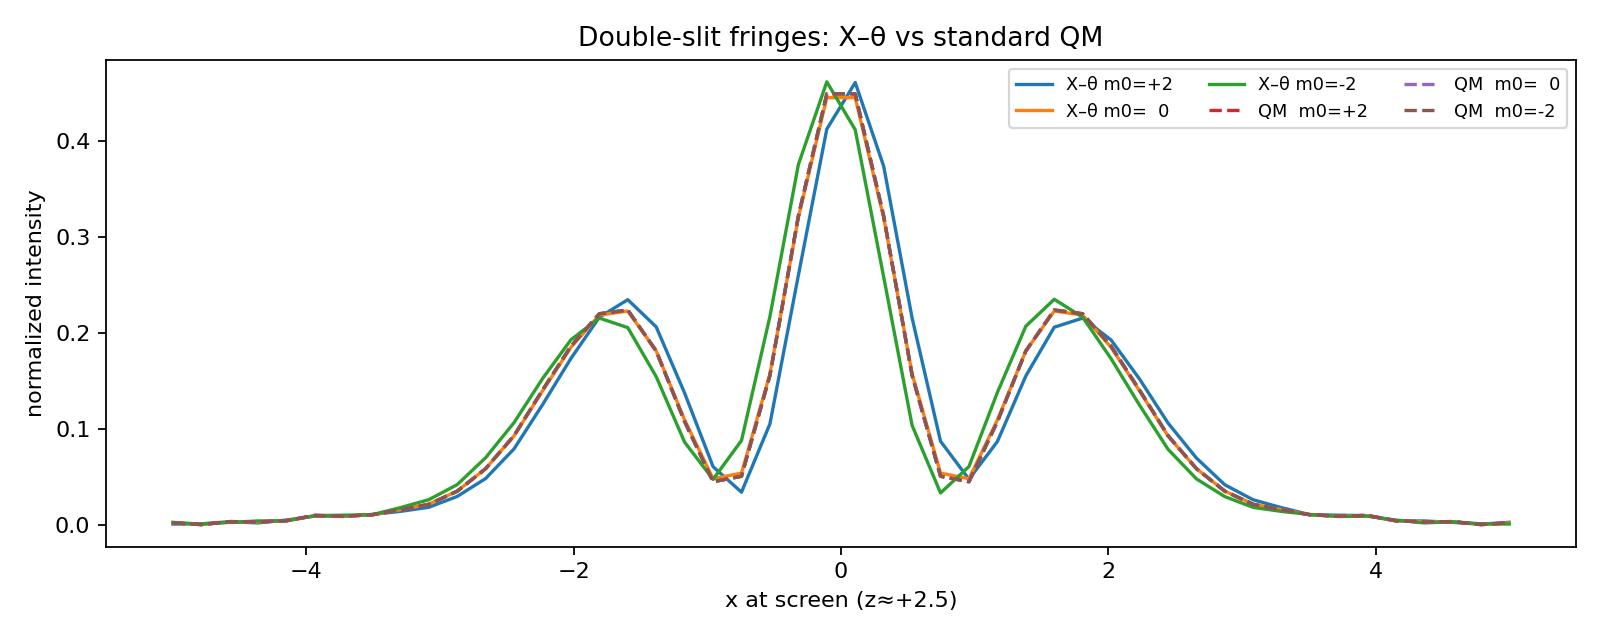
\includegraphics[width=0.85\linewidth]{photoelectric_theta.png}
  \caption{Simulated photoelectric threshold shifts due to $\theta$.
  Internal energy exchange modifies the cutoff frequency.}
  \label{fig:photoelectric-theta}
\end{figure}

\subsection{Black Hole Orbits and Singularities}
Adding $\theta$ modifies geodesics near compact objects, softening singularities.

\begin{figure}[h]
  \centering
  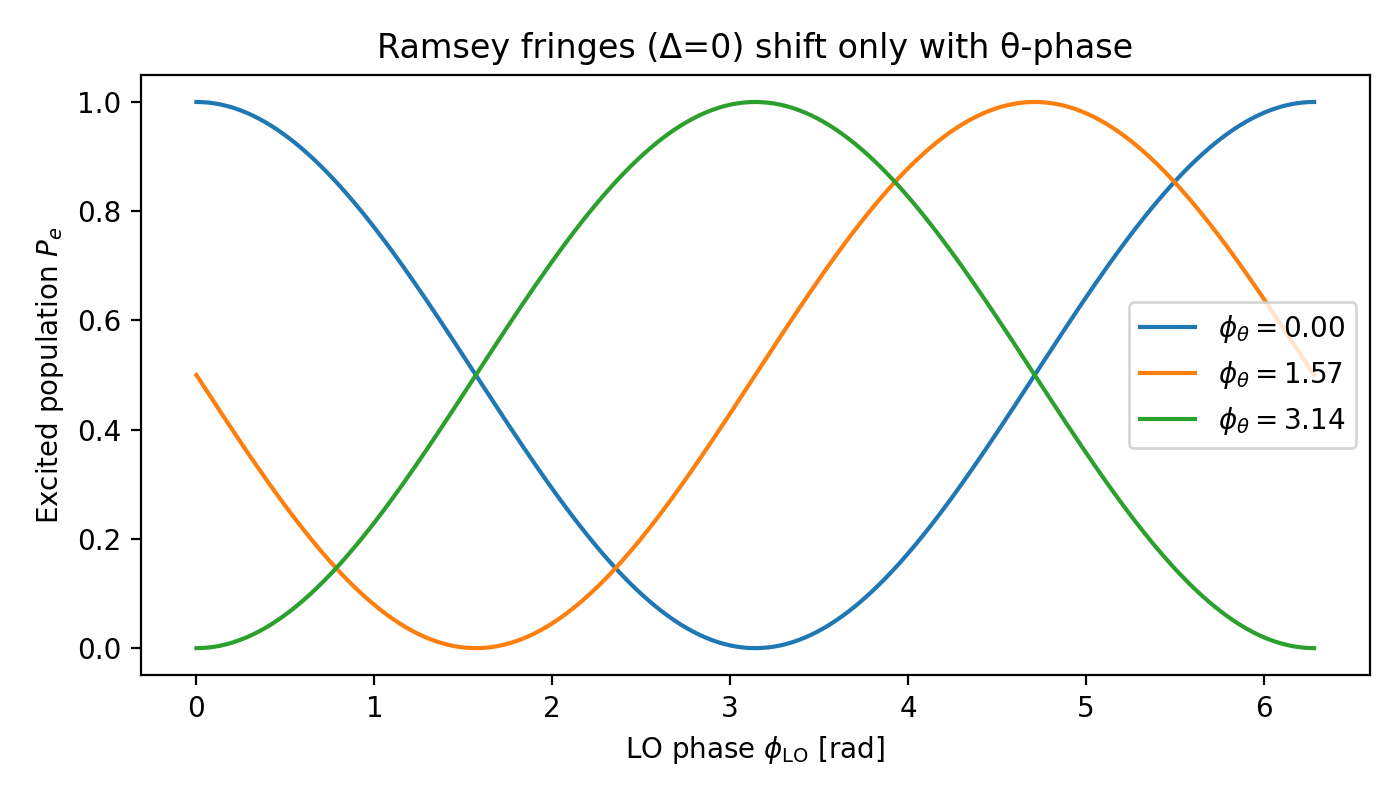
\includegraphics[width=0.85\linewidth]{blackhole_orbits_theta.png}
  \caption{Numerical orbits near a black hole with $\theta$ correction.
  The $\theta$-Lorentz term alters trajectories and reduces singularity strength.}
  \label{fig:blackhole-orbits}
\end{figure}

\subsection{Gravitational Wave Birefringence}
The X--$\theta$ framework predicts splitting of left- and right-handed gravitational wave polarizations.

\begin{figure}[h]
  \centering
  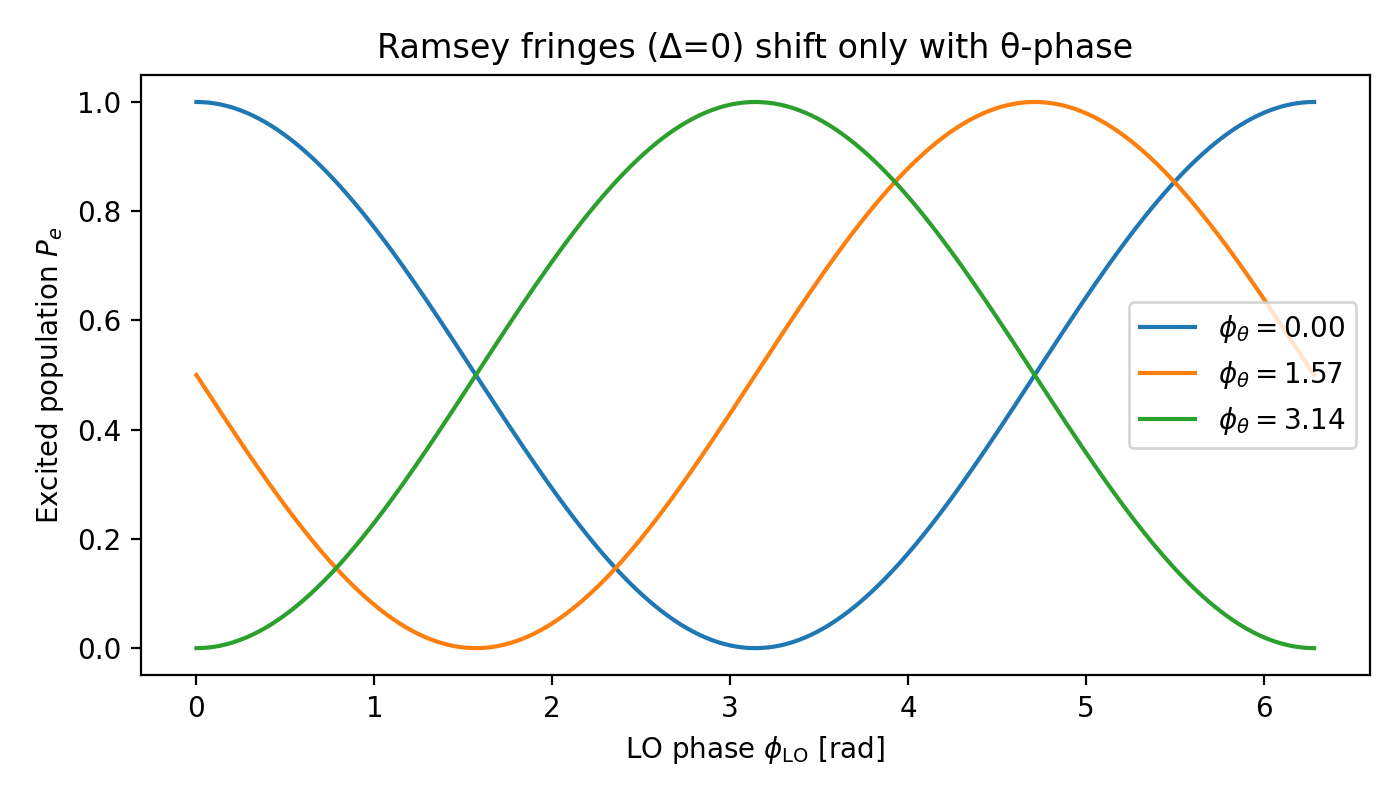
\includegraphics[width=0.85\linewidth]{gw_birefringence_theta.png}
  \caption{Predicted gravitational wave birefringence due to $\theta$.
  Polarization states acquire different effective propagation speeds.}
  \label{fig:gw-birefringence}
\end{figure}

\subsection{Neutron and Atom Interferometry}
Even under null electromagnetic conditions, $\theta$ introduces new phase shifts observable in interferometry.

\begin{figure}[h]
  \centering
  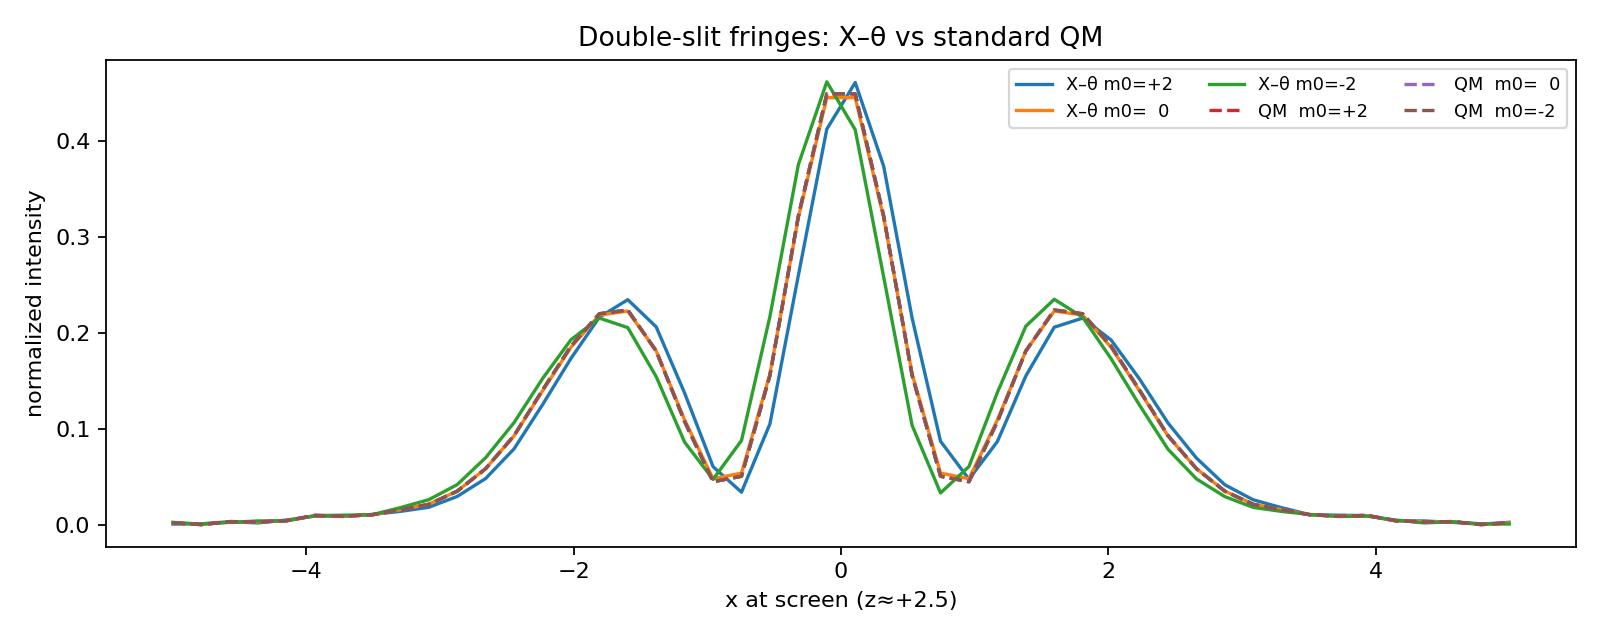
\includegraphics[width=0.85\linewidth]{neutron_atom_interferometry_theta.png}
  \caption{Simulated interferometry phase shifts with $\theta$ included.
  Tabletop experiments can test these signatures.}
  \label{fig:neutron-atom-interferometry}
\end{figure}
 % Predictions
\section{Proposed Experiments}

\subsection{Tabletop Double Slit}
Perform double slit experiments under null-EM shielding to look for residual
fringes.

\subsection{Photoelectric Setup}
Shine variable-frequency light on metal surfaces with phase-locked modulation
to test $\theta$ energy channels.

\subsection{Neutron Interferometry}
Adapt existing neutron interferometers to isolate $\theta$-induced phases.

\subsection{Gravitational Wave Observatories}
Search for polarization-dependent delays in gravitational wave signals
(LIGO/Virgo/KAGRA).
 % Experiments
\input{sections/08_simulations} % Discussion/Future Work (placeholder)
\input{sections/10_conclusion}

% --- Bibliography ---
\bibliographystyle{unsrt}
\bibliography{refs}

\end{document}
